\section{Results of Part 2}

\subsection{Question A}
The bubble sort function was created based off of sudo code for a generalised bubble sort.
The code is shown below

\begin{Matlab}
 function array = BubbleSort(array)
  for i = 1:length(array)
   for j = length(array):-1:i+1
    if array(j) > array(j-1)
     temp = array(j);
     array(j) = array(j-1);
     array(j-1) = temp;
    end
   end
  end
 return;
 end
\end{Matlab}

This code took 0.0087 seconds to sort the 100x100 matrix

\subsection{Question B}
The code to test the user function is shown below.
'timetaken' is a matrix for storing the times of both the user and inbuilt functions.

\begin{Matlab}
 % Initialize array
 testsizes = [100; 200; 500; 1000; 10000];%grid sizes tested
 timetaken = cell(1+length(testsizes),4);
 timetaken(1,:) = {"size", "bubble sort time", "inbuilt sort time", "speed up"};
 timetaken(2:end,1) = num2cell(testsizes); 

 % Loop over each row in timetaken
 for i = 2:size(timetaken,1)
  % Call the timetest function 
  %with the value in the first column (grid size) of the i-th row
  [timeBubble, timeInbuilt] = timetest(timetaken{i,1});
  timetaken{i,2} = timeBubble;
  timetaken{i,3} = timeInbuilt;
  % Calculate speed up
  timetaken{i,4} = timeBubble/timeInbuilt;
 end
 disp(timetaken)
\end{Matlab}

The function 'timetest' is given below.
It takes a matrix size, creates a square matrix, and then outputs the sort time for both the user and inbuilt functions.



\begin{Matlab}
 function [t_user,t_inbulit ] = timetest(size)

  X=rand(size, size);
  Y=X;

  tic
  for i = 1:size
   X(:,i) = BubbleSort(X(:,i));
  end
  t_user = toc();

  tic
  for i = 1:size
   Y(:,i) = sort(Y(:,i));
  end
  t_inbulit = toc();

  display("Time tacken by the bubble sort function was " + t_user " s.")
  display(" s. Time tacken by the inbuilt sort function was: "+  t_inbulit +" s.")

  return;
 end
\end{Matlab}

The results from the tests are shown in the table below

\Table{User vs inbuilt sort function}{lrrr}{
 \textbf{Matrix size} & \textbf{User} & \textbf{Inbuilt} & \textbf{Speed up}
}{
 100 & 0.0087 & 0.0002 & 40.507 \\
 200 & 0.0205 & 0.0003 & 62.791 \\
 500 & 0.1780 & 0.0012 & 145.18 \\
 1000 & 2.1324 & 0.0048 & 445.16 \\
 1000 & 1813.9 & 1.5631 & 1160.4 \\
}{2btbl}

\begin{figure}[H]
 \centering
 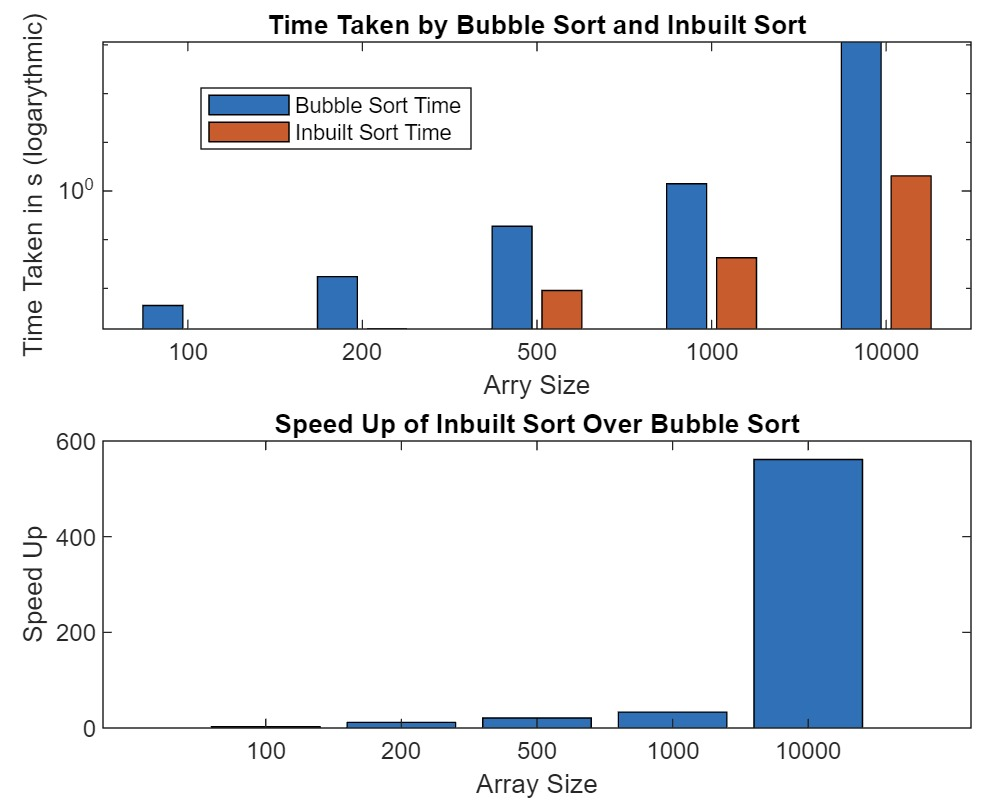
\includegraphics[width=0.6\columnwidth]{Figures/noPar}
 \caption{User vs inbuilt sort function}
 \label{fig:noPar}
\end{figure}

These results are logical because the inbuilt sort function uses the Quick Sort algorithm. ~\cite{MathWorks_Support_Team}
this means that the bubble sort function has a big O notation of $O(n^2)$, while the inbuilt sort function has a big O notation of $O(n\log(n))$ in most cases.~\cite
This means that the inbuilt sort function will be faster than the bubble sort function for all sizes.
However, the time difference will be more pronounced as the size of the matrix increases.

The speed up expected has a big O notation of $O(n^2/\log(n))$ which is $O(n/\log(n))$.
This means that the speed up will increase as the size of the matrix increases as shown in the graph below.


\begin{figure}[H]
    \centering
    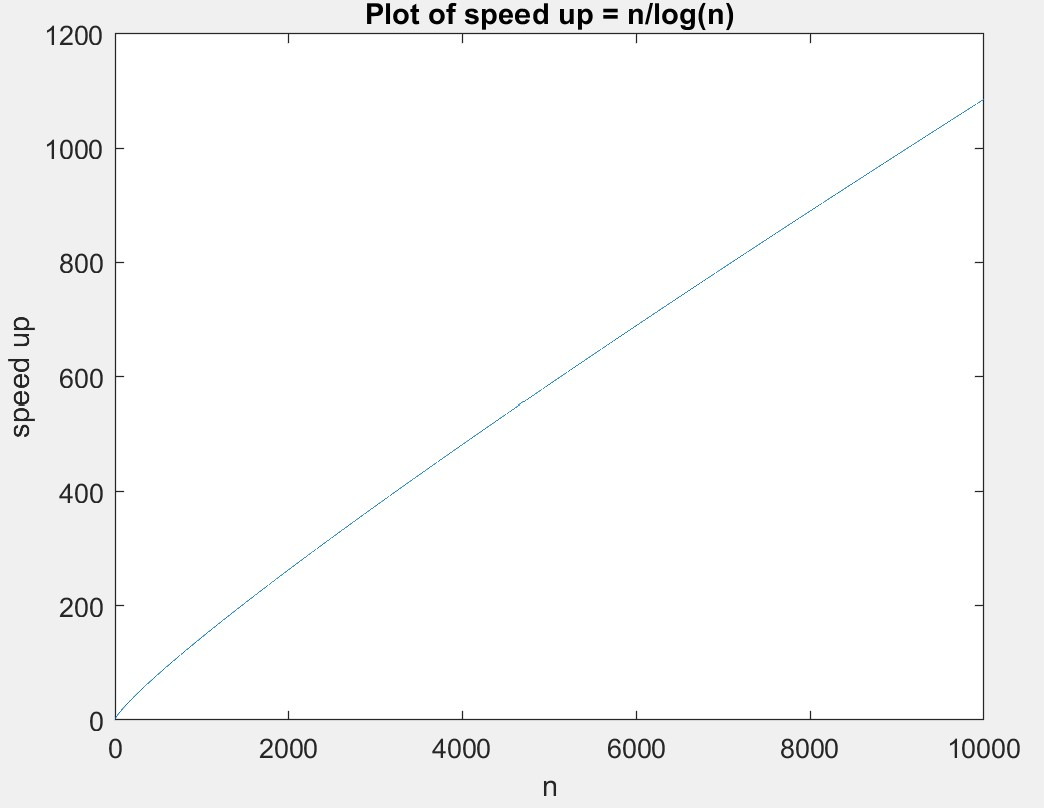
\includegraphics[width=0.6\columnwidth]{Figures/speed_up_big n notation}
    \caption{speed up big O notation}
    \label{fig:noPar}
\end{figure}

\subsection{Question C}
The code to test the parallelism  user function is shown below.
'timetaken' is a matrix for storing the times of both the user and inbuilt functions.

\begin{Matlab}
 testsizes = [100, 5000];
 timetaken_par = cell(1+length(testsizes),4);
 timetaken_par(1,:) = {"size", "bubble sort time", "inbuilt sort time", "speed up"};
 timetaken_par(2:end,1) = num2cell(testsizes); 

 % Loop over each row in timetaken_par
 for i = 2:size(timetaken_par,1)
  % Call the timetest function with the value in the first column of the i-th row
  timeBubble = timebubble_parallelism(timetaken_par{i,1});
  timeInbuilt = timesort_parallelism(timetaken_par{i,1});
  timetaken_par{i,2} = timeBubble;
  timetaken_par{i,3} = timeInbuilt;
  % Calculate speed up
  timetaken_par{i,4} = timeBubble/timeInbuilt;
 end

 % Display the results
 disp(timetaken_par)
\end{Matlab}

The function 'timesort\_parallelism' simply returns the time to sort a square matrix of a given size using the inbuilt sort function.
The function 'timebubble\_parallelism' is given below.
It takes a matrix size, creates a square matrix, and then outputs the sort time for the user parallelism bubble-sort function.

\begin{Matlab}
function t_user = timebubble_parallelism(size)
    X=rand(size, size);
    tic
    spmd
        myStart = (spmdIndex - 1) * size/4 + 1;
        myEnd = myStart + size/4-1; 
        for i = myStart:myEnd
            X(:,i) = BubbleSort(X(:,i));
        end
    end
    t_user = toc();
    
    display("Time tacken by the parallelism bubble sort function was " + t_user );
    return;
end
\end{Matlab}

The results from the tests are shown in the table below

\Table{User vs inbuilt sort function}{lrrr}{
 \textbf{Matrix size} & \textbf{parallelized BubbleSort} & \textbf{Inbuilt} & \textbf{Speed up}
}{
 100 & 0.7642 & 0.001 & 764.96 \\
 5000 & 111.7174 & 1.0715 & 104.26 \\
}{2ctbl}

\begin{figure}[H]
 \centering
 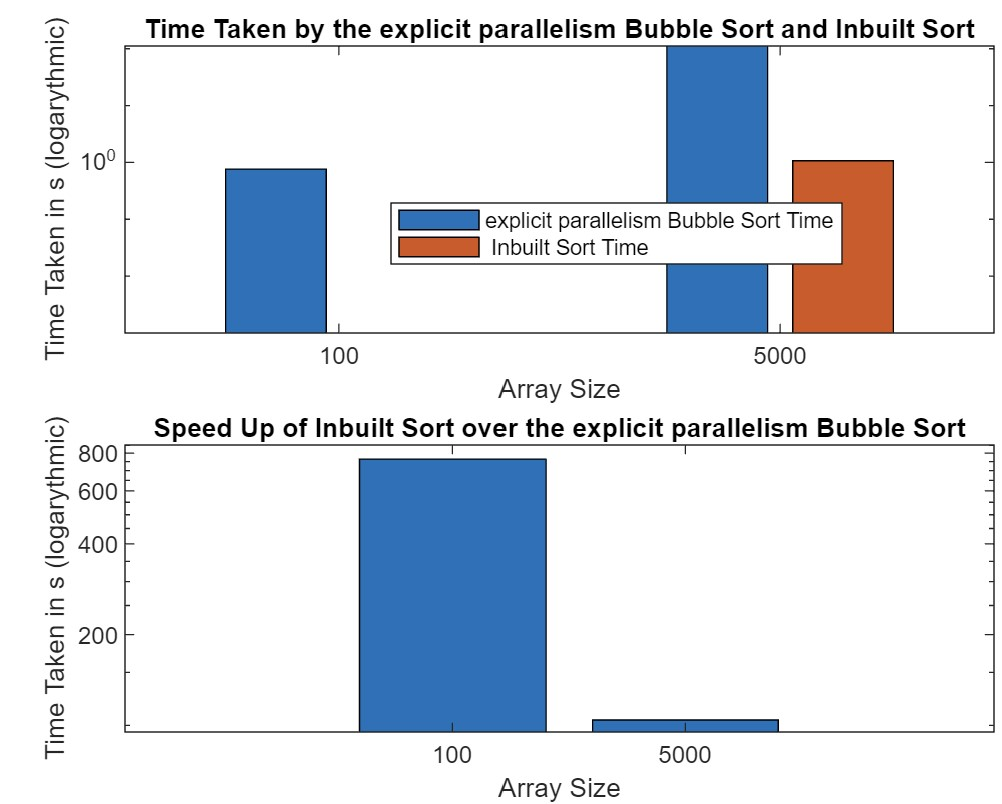
\includegraphics[width=0.6\columnwidth]{Figures/expPar_2}
 \caption{User parallelism vs inbuilt sort function}
 \label{fig:expPar}
\end{figure}

The results show that the sort function is faster than the parallelism bubble sort function.
This is because when the parallelize BubbleSort run on a nxn matrix the big O notation is $O(n×(n^2/p))$ where p is the number of workers in the parallel pool. 
The inbuilt sort function has a big O notation of $O(n×(n*log(n)))$.(There is an extra n because every column need to be sorted).

It makes sense for the speed up to slow down as the size of the matrix increases form 100 to 5000 as building the SPMD function takes time. this will hav a more noticeable effect lower-sized arrays.
